\documentclass[12pt,twocolumn]{article}
\usepackage[utf8]{inputenc}
\usepackage{amsmath,amssymb}
\usepackage{graphicx}
\usepackage{hyperref}
\usepackage{booktabs}
\usepackage{listings}
\usepackage{fancyhdr}
\usepackage{caption}
\usepackage{multicol}

% Headers and footers
\pagestyle{fancy}
\fancyhf{}
\fancyhead[L]{Comprehensive Test Document}
\fancyhead[R]{LeafPress QA}
\fancyfoot[C]{\thepage}
\fancyfoot[R]{Confidential}

% Custom macros (should warn)
\newcommand{\highlight}[1]{\textbf{#1}}
\newcommand{\eg}{e.g.}

\title{Comprehensive \LaTeX{} Feature Test}
\author{Test Author \and Second Author}
\date{January 2025}

\begin{document}
\maketitle
\tableofcontents

% --- Headings ---
\section{Headings and Structure}

\subsection{Subsection Heading}
Content under subsection.

\subsubsection{Subsubsection Heading}
Content under subsubsection.

\paragraph{Paragraph Heading}
Content under paragraph heading.

\subparagraph{Subparagraph Heading}
Content under subparagraph heading.

% --- Formatting ---
\section{Text Formatting}

This section tests \textbf{bold text}, \textit{italic text}, \emph{emphasized text},
\texttt{monospace text}, and \underline{underlined text}.

Combined formatting: \textbf{\textit{bold italic}}, \textit{\texttt{italic monospace}}.

Subscript: H\textsubscript{2}O is water. Superscript: E = mc\textsuperscript{2}.

Special characters: \& \% \$ \# \_ \{ \} \~{} \^{} \textbackslash

Unicode symbols: \copyright{} \dag{} \ddag{} \S{} \P{}

% Emoji-like symbols via math
Math symbols as decorative elements: $\star$ $\heartsuit$ $\diamondsuit$ $\clubsuit$

% --- Lists ---
\section{Lists}

\subsection{Bullet List}
\begin{itemize}
\item First bullet item
\item Second bullet item with \textbf{bold}
\item Third item
  \begin{itemize}
  \item Nested bullet A
  \item Nested bullet B
    \begin{itemize}
    \item Deep nested item
    \end{itemize}
  \end{itemize}
\item Back to top level
\end{itemize}

\subsection{Numbered List}
\begin{enumerate}
\item First numbered item
\item Second numbered item
\item Third item
  \begin{enumerate}
  \item Sub-item a
  \item Sub-item b
  \end{enumerate}
\item Back to top level
\end{enumerate}

\subsection{Description List}
\begin{description}
\item[Term One] Definition of the first term.
\item[Term Two] Definition of the second term with \emph{emphasis}.
\item[Term Three] A longer description that spans multiple
  words and explains the concept thoroughly.
\end{description}

% --- Tables ---
\section{Tables}

\subsection{Simple Table}
\begin{tabular}{|l|c|r|}
\hline
Left & Center & Right \\
\hline
Alpha & 100 & \$1.00 \\
Beta & 200 & \$2.50 \\
Gamma & 300 & \$3.75 \\
\hline
\end{tabular}

\subsection{Booktabs Table}
\begin{tabular}{lrr}
\toprule
Feature & Version 1 & Version 2 \\
\midrule
Speed (ms) & 120 & 45 \\
Memory (MB) & 512 & 256 \\
Accuracy (\%) & 92.3 & 97.8 \\
\bottomrule
\end{tabular}

% --- Math / Equations ---
\section{Equations and Math}

Inline math: The quadratic formula is $x = \frac{-b \pm \sqrt{b^2 - 4ac}}{2a}$.

Display equation:
\begin{equation}\label{eq:euler}
e^{i\pi} + 1 = 0
\end{equation}

Equation array:
\begin{align}
\nabla \cdot \mathbf{E} &= \frac{\rho}{\epsilon_0} \label{eq:gauss} \\
\nabla \times \mathbf{B} &= \mu_0 \mathbf{J} + \mu_0 \epsilon_0 \frac{\partial \mathbf{E}}{\partial t}
\end{align}

Unnumbered equation:
\begin{equation*}
\sum_{n=1}^{\infty} \frac{1}{n^2} = \frac{\pi^2}{6}
\end{equation*}

Cross-references: See Equation~\eqref{eq:euler} and Section~\ref{sec:code}.

% --- Code Blocks ---
\section{Code Blocks}\label{sec:code}

\subsection{Verbatim}
\begin{verbatim}
def hello():
    print("Hello, World!")
    return 42
\end{verbatim}

\subsection{Listings with Language}
\begin{lstlisting}[language=Python]
import numpy as np

def fibonacci(n: int) -> list[int]:
    """Generate Fibonacci sequence."""
    fib = [0, 1]
    for i in range(2, n):
        fib.append(fib[-1] + fib[-2])
    return fib[:n]
\end{lstlisting}

% --- Hyperlinks ---
\section{Hyperlinks}

Visit \href{https://example.com/docs}{the documentation page} for details.

The source code is at \url{https://github.com/example/project}.

See \href{https://example.com/api}{API Reference} and
\href{https://example.com/changelog}{Changelog}.

% --- Figures / Images ---
\section{Figures and Captions}\label{sec:figures}

\begin{figure}[htbp]
\centering
\includegraphics{test_figure.png}
\caption{A test figure demonstrating image import with caption support.}
\label{fig:test}
\end{figure}

See Figure~\ref{fig:test} for the visualization.

% --- Blockquotes ---
\section{Blockquotes}

\begin{quote}
The best way to predict the future is to invent it. --- Alan Kay
\end{quote}

\begin{quotation}
This is a longer quotation that spans multiple sentences. It is used to
demonstrate the quotation environment, which is similar to quote but
with paragraph indentation. This is a common feature in academic documents.
\end{quotation}

% --- Footnotes ---
\section{Footnotes}

This sentence has a footnote\footnote{This is the first footnote with
\textbf{bold} and \textit{italic} formatting.}.

Here is another\footnote{Second footnote referencing a \href{https://example.com}{link}.}.

And a third\footnote{Third footnote with math: $E = mc^2$.}.

% --- Citations ---
\section{Citations and References}

As shown by \cite{knuth1984}, typesetting is an art form.
Multiple citations \cite{lamport1994,knuth1984} are supported.
Author-year style: \citet{dijkstra1968} proved this.

% --- Table of Contents reference ---
\section{Cross-References}

See Section~\ref{sec:code} for code examples.
See Section~\ref{sec:figures} for figures.
See Equation~\eqref{eq:euler} for Euler's identity.
See Equation~\eqref{eq:gauss} for Gauss's law.

% --- Page break ---
\newpage

% --- Section break (new section after page break) ---
\section{Final Section After Page Break}

This section appears after a page break, testing section break behavior.

% --- Nested environments ---
\begin{center}
This text is centered.
\end{center}

\begin{minipage}{0.8\textwidth}
This is inside a minipage environment with constrained width.
\end{minipage}

% --- Unsupported environments (should warn) ---
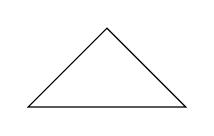
\begin{tikzpicture}
\draw (0,0) -- (1,1) -- (2,0) -- cycle;
\end{tikzpicture}

% --- Bibliography ---
\begin{thebibliography}{99}
\bibitem{knuth1984} Donald E. Knuth, \emph{The \TeX{}book}, Addison-Wesley, 1984.
\bibitem{lamport1994} Leslie Lamport, \emph{\LaTeX{}: A Document Preparation System}, 2nd ed., Addison-Wesley, 1994.
\bibitem{dijkstra1968} Edsger W. Dijkstra, ``Go To Statement Considered Harmful,'' \emph{Communications of the ACM}, 11(3):147--148, 1968.
\end{thebibliography}

\end{document}
